\ItemCategory{}
\ItemSubCategory{}
\ItemFolder{}

\chapter*{Crossbow of the Deep Ones}\stepcounter{section}\phantomsection\addcontentsline{toc}{section}{Crossbow of the Deep Ones}
\itemDescriptionAndImage{Wondrous Crossbow, Artifact (requires attunement by an Aberrant Mind Sorcerer or Fathomless Warlock)}{images/Magic_Items/Crossbow_of_the_Deep_Ones.png}{6.5cm}\\

\begin{tikzpicture}[remember picture, overlay]%
	\node[xshift=0.55\columnwidth, yshift=-0.35\paperheight] at (current page.center) {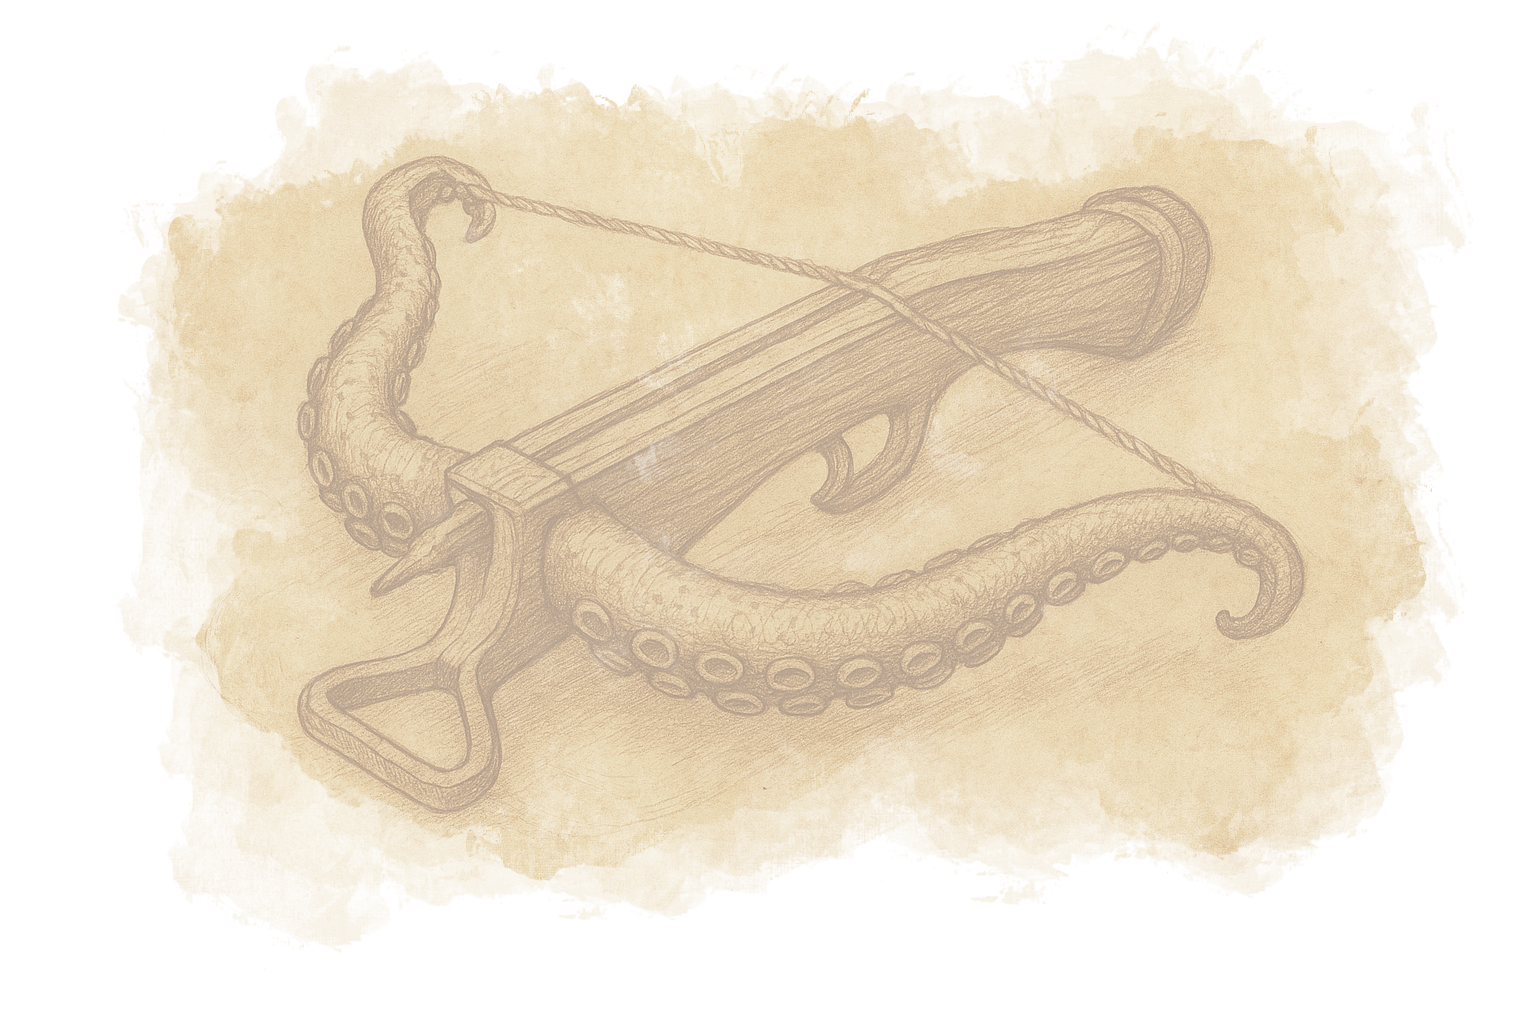
\includegraphics[width=1.6\columnwidth]{%
		images/Magic_Items/Crossbow_of_the_Deep_Ones_background.png%
	}};%
\end{tikzpicture}%

\section*{Appearance}
{\entryfont The Crossbow of the Deep Ones is a grotesque yet masterfully crafted weapon, its design straddling the line between mortal craftsmanship and something born from the abyss. The stock is fashioned from dark, sea-worn wood, its grain etched with barnacle-like ridges and faint whorls resembling coral. Metallic inlays, tarnished as if by saltwater, reinforce its frame and gleam faintly under the light.

Its most striking feature is the prod: a pair of arms that are unmistakably shaped like kraken tentacles. Each arm curls outward in a natural arc, textured with ridges and lined with sucker-like impressions that glisten with an unsettling, almost organic realism. These tentacle-arms give the crossbow a sense of being alive, as though it might writhe if not bound by string and wood.}
\section*{History}
{\entryfont The origins of the Crossbow of the Deep Ones are shrouded in murky waters, with no records of its creation found in any mortal archive. Sailors whisper that the weapon surfaces only when the veil between the seas and the abyss thins. Its appearance is said to coincide with sightings of abyssal horrors and twisted aberrations rising from the depths.

Those who claim to have seen it describe it as more summoned than forged, called forth by the will of powers lurking in the blackest trenches. Some coastal hunter lodges believe it was once wielded by a mortal who bargained with the deep, while others insist it is a weapon of the Deep Ones themselves, left behind as a harbinger of their approach. Whatever its truth, wherever the crossbow is found, calamity is rarely far behind.}
\vfill\eject
\section*{Magic}
{\entryfont The Crossbow of the Deep Ones is more than a weapon - it is a conduit for abyssal dread. Bolts fired from it are infused with a fragment of the horror that dwells beneath the waves. On impact, victims may feel their minds assaulted by visions of the fathomless deep, suffering searing psychic pain as if they had glimpsed the alien will of the abyss itself.

At other times, the crossbow's power manifests more tangibly. From the point of impact, writhing tentacles of brine-soaked shadow erupt, coiling around the target to restrain them or lashing violently to rend flesh and bone. Witnesses say these manifestations leave behind a lingering dampness and the faint imprint of suckers, as though something vast and unseen briefly reached through from the ocean's blackest depths.}
\subsection*{Gameplay Mechanics}
{\entryfont
\subsubsection*{Dormant State}
\begin{itemize}
	\item The wielder gains a +1 bonus to attack and damage rolls made with this weapon.
	\item When the wielder hits with an attack using this weapon, the target takes an additional 1d4 Psychic damage.
	\item If the wielder hits with an attack using this weapon, instead of dealing damage, they can choose to release the wrath of the Deep Ones, choosing one of the following effects (Spell Save DC 12):
	\begin{itemize}
		\item An Arms of Hadar Spell centered on the target (target is also affected)
		\item A Silence Spell centered on the target.
	\end{itemize}
	No concentration is required to uphold the effects, however, only one of the effects can be active at one time. This feature can be used a number of times equal to the wielder's Charisma modifier value (minimum of 1), and all expended uses are regained when finishing a long rest.
\end{itemize}
\subsubsection*{Awakened State}
\begin{itemize}
	\item The bonus to attack and damage rolls increases to a +2.
	\item The Psychic damage dealt by attacks with this weapon increases to 1d6.
	\item The Spell Save DC of the triggered effects increases to 14.
	\item Additional effects can be triggered instead of damage:
	\begin{itemize}
		\item A Hold Person Spell.
		\item A Hunger of Hadar Spell centered on the target.
	\end{itemize}
\end{itemize}
\subsubsection*{Exalted State}
\begin{itemize}
	\item The bonus to attack and damage rolls increases to a +3.
	\item The Psychic damage dealt by attacks with this weapon increases to 1d8.
	\item The Spell Save DC of the triggered effects equals the wielder's Spell Save DC.
	\item Additional effects can be triggered instead of damage and two effects can be active simultaneously:
	\begin{itemize}
		\item A Bigby's Hand Spell (appears as a tentacle) located in an unoccupied space next to the target.
	\end{itemize}
\end{itemize}}
\vfill\eject
\DndSpellHeader
  {Arms of Hadar}
  {1st-Level Conjuration}
  {Action}
  {Self}
  {V, S}
  {Instantaneous}

\noindent Each creature in a 10-foot Emanation originating from you makes a Strength saving throw. On a failed save, a target takes 2d6 Necrotic damage and can't take Reactions until the start of its next turn. On a successful save, a target takes half as much damage only.

\DndSpellHeader
  {Silence}
  {2nd-Level Illusion}
  {Action}
  {120 Feet}
  {V, S}
  {Concentration, Up to 10 Minutes}

\noindent For the duration, no sound can be created within or pass through a 20-foot-radius Sphere centered on a point you choose within range. Any creature or object entirely inside the Sphere has Immunity to Thunder damage, and creatures have the Deafened condition while entirely inside it. Casting a spell that includes a Verbal component is impossible there.

\DndSpellHeader
  {Hold Person}
  {2nd-Level Enchantment}
  {Action}
  {60 Feet}
  {V, S, M (a straight piece of iron)}
  {Concentration, Up to 1 Minute}

\noindent Choose a Humanoid that you can see within range. The target must succeed on a Wisdom saving throw or have the Paralyzed condition for the duration. At the end of each of its turns, the target repeats the save, ending the spell on itself on a success.

\DndSpellHeader
  {Hunger of Hadar}
  {3rd-Level Conjuration}
  {Action}
  {150 Feet}
  {V, S, M (a pickled tentacle)}
  {Concentration, Up to 1 Minute}

\noindent A 20-foot-radius Sphere of Darkness appears, centered on a point within range and lasting for the duration. The Sphere is Difficult Terrain, and it is filled with strange whispers and slurping noises, which can be heard up to 30 feet away. No light, magical or otherwise, can illuminate the area, and creatures fully within have the Blinded condition.

Any creature that starts its turn in the area takes 2d6 Cold damage. Any creature that ends its turn there must succeed on a Dexterity saving throw or take 2d6 Acid damage from otherworldly tentacles.0

\DndSpellHeader
  {Bigby's Hand}
  {5th-Level Evocation}
  {Action}
  {120 Feet}
  {V, S, M (an eggshell and a glove)}
  {Concentration, Up to 1 Minute}

You create a Large hand of shimmering, translucent force in an unoccupied space that you can see within range. The hand lasts for the spell's duration, and it moves at your command, mimicking the movements of your own hand.

The hand is an object that has AC 20 and Hit Points equal to your Hit Point maximum. If it drops to 0 Hit Points, the spell ends. The hand doesn't fill its space.

When you cast the spell and as a bonus action on your subsequent turns, you can move the hand up to 60 feet and then cause one of the following effects with it.

\paragraph*{Clenched Fist} The hand strikes a target within 5 feet of it. Make a melee spell attack. On a hit, the target takes 5d8 Force damage.
\paragraph*{Forceful Hand} The hand attempts to push a Huge or smaller creature within 5 feet of it. The target must succeed on a Strength saving throw, or the hand pushes the target up to 5 feet plus a number of feet equal to five times your spellcasting ability modifier. The hand moves with the target, remaining within 5 feet of it.
\paragraph*{Grasping Hand} The hand attempts to grapple a Huge or smaller creature within 5 feet of it. You use the hand's Strength score to resolve the grapple. If the target is Medium or smaller, you have advantage on the check. While the hand is grappling the target, you can take a Bonus Action to cause the hand crush it. When you do so, the target takes bludgeoning damage equal to 4d6 + your spellcasting ability modifier.
\paragraph*{Interposing Hand} The hand grants you Half Cover against attacks and other effects that originate from its space or that pass through it. In addition, its space counts as Difficult Terrain for your enemies.